\section{IntelliJ IDEA}
\author{Benjamin Besic}

IntelliJ IDEA ist eine der führenden Entwicklungsumgebungen für die Programmiersprache Java. Sie wurde vom Unternehmen Jetbrains im Jahre 2000 entwickelt.
\\* Außerdem bietet sie ebenfalls Entwicklungsmöglichkeiten für Kotlin, Groovy, Scala und auch Android.
 Sie ist immer auf dem neusten Entwicklungsstand, wird laufend mit Updates versorgt und unterstützt die derzeit gängigen Programmiertools
wie Docker, Kubernetes, Maven, Datenbank-Tools, Git, Jakarta EE und viele weitere.
Es gibt eine kostenpflichtige Ultimate Version und eine Community Version, die kostenfrei zur Verfügung gestellt wird.
\\* IntelliJ zeichnet auch die Anzahl an Erweiterungen mittels Plugins aus. Die Umgebung besitzt auch eine
sehr intuitive Intelligenz, die es dem Entwickler sehr einfach macht damit zu programmieren.
\cite{IntJ} \\*
Wir haben uns dafür entschieden, da wir damit viel Erfahrung hatten und die oben genannten Punkte
unterstützten unsere Entscheidung enorm.

\section{Android Studio}

\section{Git}
\author{Benjamin Besic}
Git ist ein Versionskontrollsystem (oft abgekürzt durch VCS) für Entwickler. Es ist ein Open-Source System, das im Jahre 2005
von Linus Torvald entwickelt wurde. Laut einer Stack Overflow-Umfrage von Entwicklern nutzen über 87 \% der Entwickler Git.
\cite{GitKinsta}
\\* Zu aller erst muss man den Begriff Versionskontrolle erklären, um Git zu verstehen.
\subsection{Versionskontrolle}
Diese dient dazu, um den originalen Quellcode effizient mit mehreren Personen editieren bzw. entwickeln zu können. 
\\* Die Entwickler arbeiten mit Verzweigungen und Zusammenführungen. Jeder Entwickler kann Änderungen sicher durchführen, ohne seine Kollegen dabei 
zu behindern. Diese Änderungen können dann, sobald sie funktionsfähig sind, wieder in den Hauptquellcode eingebunden werden.
Alle Änderungen sind zurückzuverfolgen und bei Bedarf kann man sie dann wieder zurücksetzen.
\cite{GitKinsta} \\*

\subsection{Git Funktionsweise}
Jeder Entwickler hat seine eigene Version des Projekts (Working Directory), die er frei bearbeiten kann. Diese bekommt man durch einen Klon des Projekts (\hyperref[sec:Clone]{Clone}). \\* Diese Änderungen kann man aufteilen und 
in Paketen bereitstellen, nach dem man diese durch Commits trennt. Einen \hyperref[sec:Commit]{Commit} kann man benennen. \\*
Diese Commits kann man dann online veröffentlichen durch einen \hyperref[sec:Push]{Push}. Ein Push ist nur möglich, wenn man die aktuellste Version des Projekts
auf seinen Rechner gezogen hat (\hyperref[sec:Pull]{Pull}). 
Einem Push kann man einen bestimmten Zweig (\hyperref[sec:Branch]{Branch}) zuordnen. 
\begin{figure}[htp]
    \author{David Ignjatovic}
    \centering
    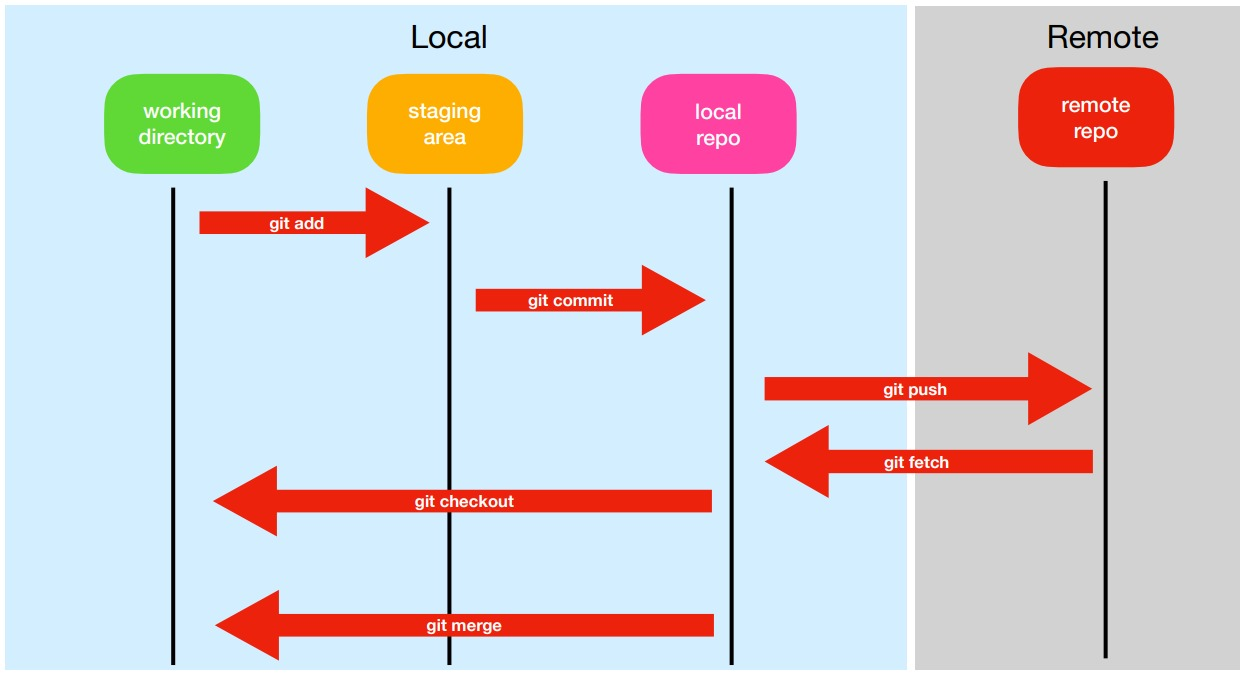
\includegraphics[scale=0.35]{pics/GitWorkflow.jpg}
    \caption{Darstellung des Git Workflows}
    \label{fig:impl:GitWorkflow}
\end{figure}
Diese Zweige dienen dazu, um das Projekt in verschiedene
unabhängige Teile zu trennen, falls man zum Beispiel an einer Demo Version weiterschreiben möchte. \\* Nach einem erfolgreichen Push sind die Änderungen
online auf dem Repository zu finden. Ein Repository ist der "Ordner", wo alle Dateien online gespeichert zu finden sind. 
\\* Ein Vorteil, den Git ebenfalls bietet ist das jeder Commit eine Version des Projekts ist, die man bis zum Zeitpunkt vom Commit herunterladen oder klonen kann.
Jedes Projekt kann privat oder öffentlich gemacht werden, sodass auch Personen, die keine Entwickler sind, darauf zugreifen können.
\cite{GitExpl} 



\subsection{Git Befehle}

\subsubsection{Clone}
\label{sec:Clone}
Es initialisiert ein Git Repository auf dem Rechner und ladet die zugehörigen Dateien runter.
Wenn man es nicht spezifisch angibt, klont es den Master Branch. Der Master Branch ist der Hauptzweig, eines jeden Git Projekts.
Innerhalb des erstellten Ordners können alle weiteren Git Befehle ausgeführt werden. \cite{GitCmnds}
\subsubsection{Commit}
\label{sec:Commit}
Ein Commit beschreibt Änderungen, die man im Projekt gemacht hat. Jeder Commit hat eine Bezeichnung, mit der der Entwickler die Änderungen,
die er gemacht hat beschreiben kann. Zu jedem Commit gehören auch die Dateien die dabei geändert bzw. hinzugefügt wurden.
\\* Es speichert den Zustand des gesamten Projekts bis zu dem Zeitpunkt und kann danach jederzeit abgerufen oder rückgängig gemacht werden.
Diese Änderungen bleiben aber zunächst nur lokal auf dem Rechner. \cite{GitCmnds}

\subsubsection{Push}
\label{sec:Push}

Ein Push dient dazu, um die lokalen Änderungen (Commits) zu veröffentlichen. Es kopiert den aktuellen, lokalen Stand und speichert diesen auf 
das vom Internet erreichbare Repository. \\* Einem Push kann ein Zweig (Branch) zugeordnet werden um die Änderungen zuzuordnen. 
Ansonsten wird der Master Branch genommen. \cite{GitCmnds}

\subsubsection{Pull}
\label{sec:Pull}
Der Pull Befehl kopiert die Inhalte vom öffentlichen Repository und fasst diese mit den lokalen Zustand auf dem 
rechner zusammen (merge). Es dient dazu die aktuelle Version des Projekts auf den Rechner herunterzuladen.
\\* Falls es Konflikte zwischen der derzeitigen und neusten Version gibt, werden die Änderungen zusammengeführt. \cite{GitCmnds}

\subsubsection{Branch}
\label{sec:Branch}
Die Branch Befehle dienen dazu um eine neue Abzweigung des Projekts (Branch) zu erstellen.
\\*
Branches erstellt man, wenn man an einer neuen Version des Projekts arbeitet und diese vom Hauptteil trennen will.
Meistens werden dadurch neue Funktionen programmiert, die später wieder in den Master Branch eingebunden werden.
\\* Der Vorteil daran ist, dass man an neuen Funktionalitäten experimentieren kann, ohne den Hauptentwicklungsstand zu 
beeinflussen. Branches können jederzeit gelöscht oder wieder ins Hauptprojekt integriert werden.
Es kann simultan am Master Branch und an Nebenzweigen gearbeitet werden durch trennen mit dem Push Befehl. \cite{GitExpl}

\begin{figure}[htp]
    \author{David Ignjatovic}
    \centering
    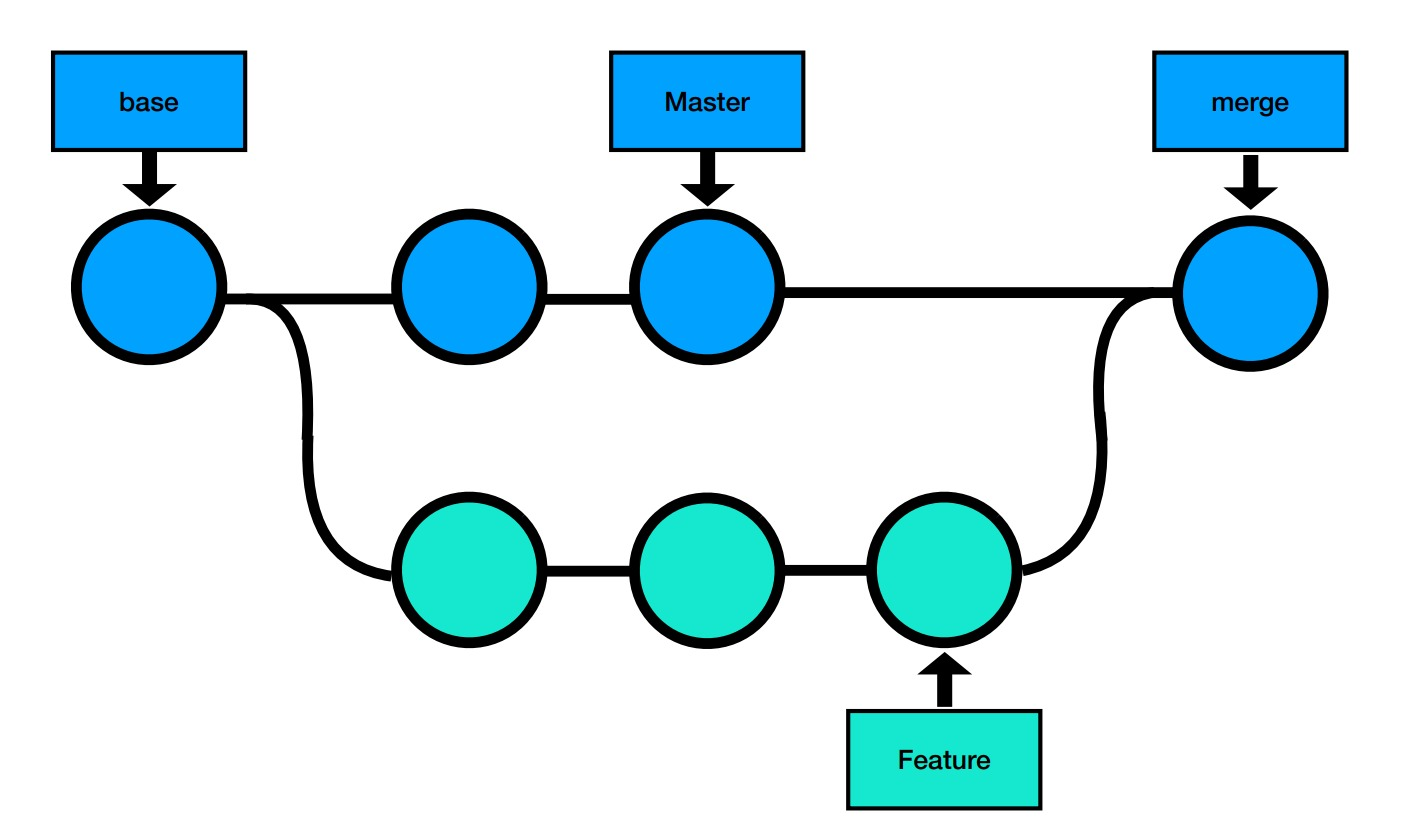
\includegraphics[scale=0.3]{pics/GitBranches.jpg}
    \caption{Darstellung von Branches in einem Repository}
    \label{fig:impl:GitBranches}
\end{figure}

\subsection{GitHub}
GitHub ist ein gewinnorientiertes Unternehmen, dass einen auf Cloud basierten Git Repository Hosting-Service anbietet.
Es wurde im Februar 2008 gestartet und von Chris Wanstrath, PJ Hyett, Scott Chacon und Tom Preston-Werner entwickelt.
Es ist das beliebteste Tool um Softwareprojekte zu verwalten und wird von über 73 Millionen Entwicklern und über 4 Millionen Organisationen
benutzt. Dazu ist es das größte und am meisten fortgeschrittene Entwicklungssystem, das es gibt. \cite{GitHub} \\*
Es vereinfacht die Nutzung von Git für Teams und auch Einzelpersonen. 
Jeder kann sich einen GitHub Account erstellen und direkt loslegen und seine Arbeiten auf Repositories veröffentlichen.
Es ist nicht nur zwingend für Code-basierte Projekte verwendbar sondern auch Websiten erstellen und das Schreiben von Büchern ist möglich.
\\*
Was GitHub ausmacht ist die Benutzerfreundlichkeit und die Integration von Git. Außerdem bietet Github viele andere Funktionen wie zum Beispiel ein Projekt Board an,
was es erleichtert innerhalb eines Teams, Probleme besser lösen zu können. \\*
Es gibt ebenfalls bezahlte Pläne, die es vor allem Organisationen und Unternehmen leichter macht Unternehmensprojekte zu verwalten durch zusätzliche Funktionen.
\cite{GitKinsta}



\section{Java}

\section{Java EE}
\subsection{Java EE vs. Quarkus}

\subsection{JPA}

\section{Quarkus}
\subsection{Hibernate}

\subsection{Panache}

\section{Maven}

\section{JBoss}

\section{Cypress}

\section{Keycloak}
\author{Benjamin Besic}
Keycloak ist eine Open-Source Software, die Single-Sign On mit Identity und Access Management für moderne Applikationen bereitstellt. Der erste Release war 2014 als Wildfly Community Projekt, seit 2018 aber steht es unter der Verwaltung von RedHat. \cite{KeycloakWiki}  \\* 
Es hat mehrere Distributionen und ist mit einer Vielzahl von Frameworks und Tools kompatibel wie z.B.: Quarkus, Angular, Vue.js, Spring, usw. \cite{KeyCloakDZone}

\subsection{Distributionen}
\subsubsection{Server}
Die Standalone Applikation ist downloadbar als .zip auf der Keycloak Seite. Es gibt zwei Versionen vom Server, zu einem die Wildy Application Server Version und auch eine Version, die über Quarkus läuft.
\subsubsection{Docker Image}
Genau so wie beim Server gibt es auch hier zwei verschiedene, offizielle Docker-Images, eins, dass auf dem Wildfly Server basiert und eins, dass auf Quarkus basiert.
\subsubsection{Operator}
Dies ist eine Distribution für Kubernetes und OpenShift, basierend auf der Operator SDK. \cite{KeyCloakDZone}
\subsection{Features}

\section{Oracle Datenbank}
\section{Vue.js}
\author{Benjamin Besic}
Vue.js ist ein JavaScript-Webframework, das zum Erstellen von Single-Page-Webanwendungen dient. 
Es wurde von einem kleinen Team im Jahre 2014 entwickelt mit dem ursprünglichem Autor Evan You.\\* Vue ist relativ neu und die große Stärke
von Vue ist die einfache Lernkurve, die Vielseitigkeit und die Leichtgewichtigkeit. Man benötigt Kenntnisse in JavaScript, HTML, CSS und schon kann man loslegen
mit deren ausführlich dokumentierten Guide\cite{VueGuide}. \cite{VueWissen} \cite{VueWiki}\\*

\subsection{Vue Funktionsweise}

\subsubsection{Model-View-Viewmodel (MVVM) Pattern }
Vue.js benutzt das MVVM Pattern. Das Pattern trennt die Darstellung von der Logik der Benutzer-UI's.
Dazu ist ein Datenbindungsmechanismus vorausgesetzt. Dadurch können sich Entwickler und Interfacedesigner trennen und ihre Aufgaben im Projekt 
aufteilen. \\*
Dieses Pattern wurde 2005 von John Gossman veröffentlicht. \cite{MVVM}

\begin{figure}[htp]
    \centering
    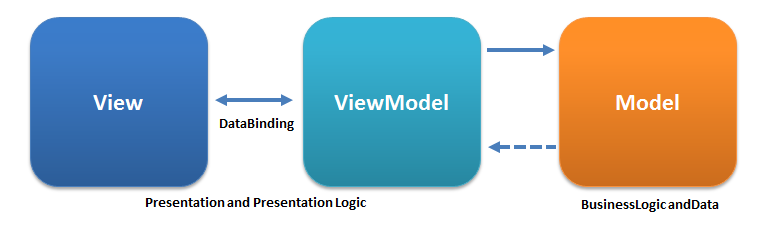
\includegraphics[scale=0.7]{pics/MVVMPattern.png}
    \caption{Darstellung von Branches in einem Repository}
        \small \url{https://upload.wikimedia.org/wikipedia/commons/8/87/MVVMPattern.png}
    \label{fig:impl:MVVM}
\end{figure}

\begin{itemize}
    \item \textbf{View:} Enthält alle Elemente die durch die Benutzeroberfläche angezeigt werden. Es bindet sich an das ViewModel, welches die Eigenschaften der View bestimmt.
    \item \textbf{ViewModel:} Es enthält die Logik des UI's. Es tauscht sich mit dem Model aus und benützt seine Methoden und Dienste. Gleichzeitig
          gibt es der View Eigenschaften, die dem Model entsprechen. Es bindet Daten mit der View und sich selbst (DataBinding).
    \item \textbf{Model:} Diese Schicht enthält alle Daten die der Benutzer manipuliert oder aufruft. Es enthält die gesamte Geschäftslogik.\cite{MVVM}
\end{itemize}

\clearpage

\subsubsection{Vue Instance}

Jede Vue Applikation beginnt mit der Erstellung einer Vue Instanz.

\begin{lstlisting}[language=JavaScript,caption=Vue Instanz,label=lst:impl:foo]
    var vm = new Vue({
        // options
    }) 
\end{lstlisting}

Die Variable vm steht für ViewModel, was unsere Vue Instanz darstellt. Man kann jeder Instanz Optionen zuweisen, um sie zu konfigurieren.
Diese Instanz wird auch als Root Instanz bezeichnet und bildet den Stamm eines Baumes mit Komponenten. 

\begin{figure}[htp]
    \centering
    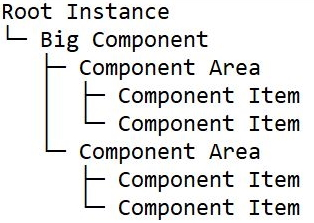
\includegraphics[scale=1]{pics/RootComponentTree.JPG}
    \caption{Der Stammbaum einer Root Instanz}
    \label{fig:impl:RootComponentTree}
\end{figure}
Zu einer Instanz gehört auch der data-Bereich. Dieser beherbergt alle Properties einer
Instanz und diese Properties reagieren auf Veränderungen im Code. Noch dazu kann jede Instanz Methoden haben. \\*
Jede Instanz hat auch seine Lifecycle Hooks, dies sind Methoden, die zu bestimmten Zeitpunkten einer Instanz ausgeführt werden. \cite{VueGuideInstance}
Diese sind:
\begin{itemize}
    \item \textbf{created}
    \item \textbf{mounted}          
    \item \textbf{updated} 
    \item \textbf{destroyed} 
\end{itemize}
\clearpage

\subsubsection{Lifecycle Diagram}
Das Diagramm hier stellt den Ablauf einer Erstellung einer neuen Vue Instanz dar.

\begin{figure}[htp]
    \centering
    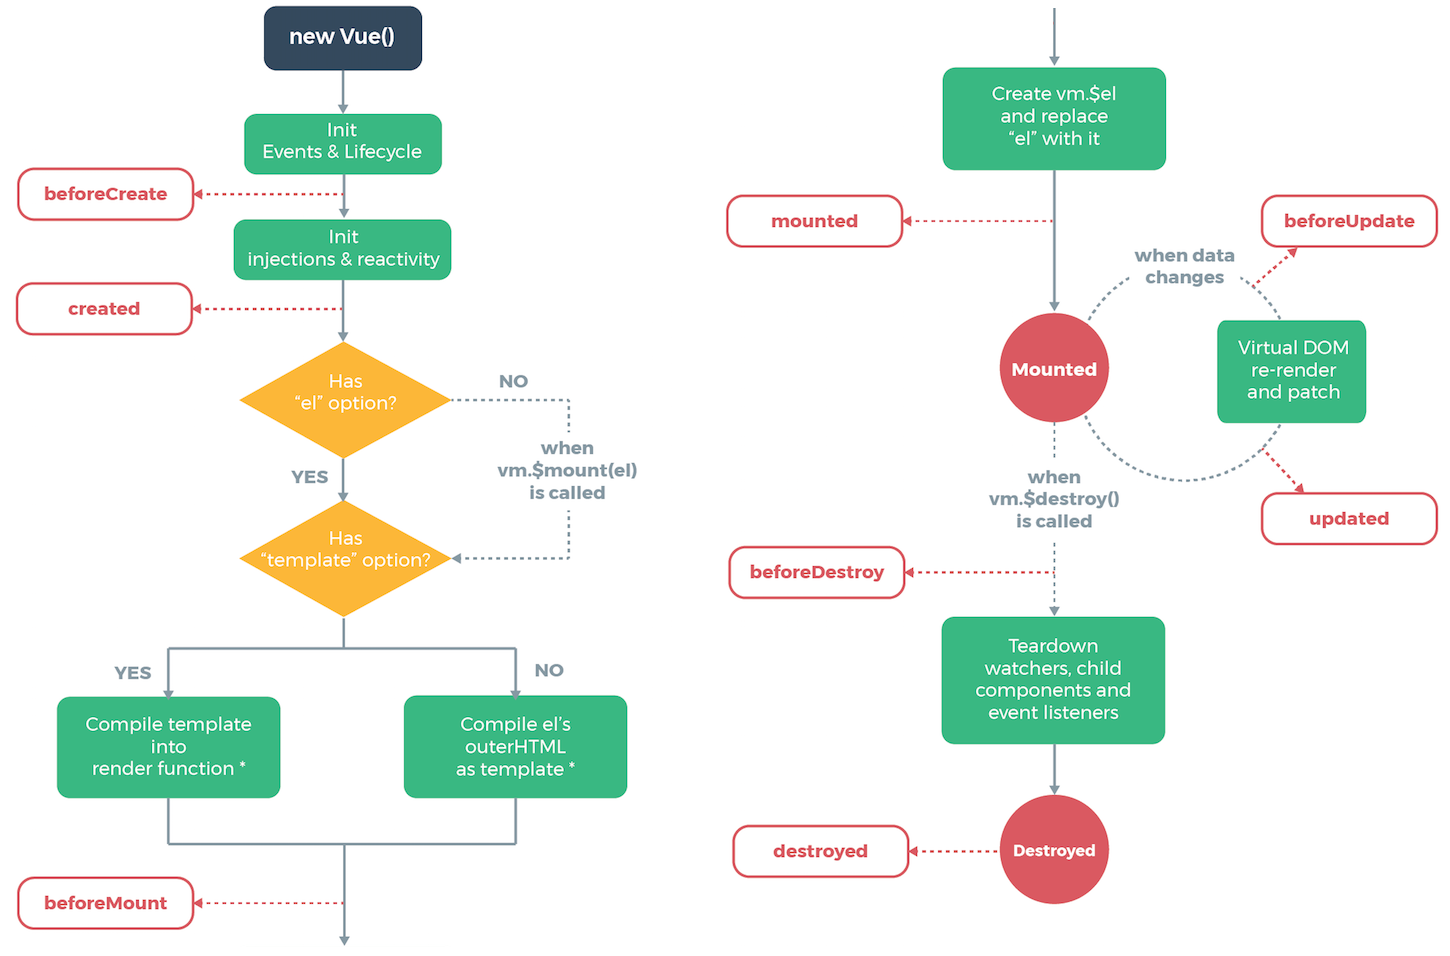
\includegraphics[scale=0.3]{pics/VueInstanceLifeCycle.png}
    \caption{Diagramm des Ablaufs einer Vue Instanz}
        \small \url{https://www.oreilly.com/library/view/full-stack-vuejs-2/9781788299589/assets/9f308e86-bbbe-489c-9f93-06abe2675081.png}
    \label{fig:impl:VueInstanceLifeCycle}
\end{figure}


\subsubsection{Vue Components}
Komponenten sind wiederverwendbare Vue Instanzen mit einem eigenen Namen. Diese Komponenten können mittels HTML-Tags in anderen Komponenten verwendet werden.
Eine Vue.js Seite ist meistens in mehrere Komponenten aufgeteilt, um größere Bereiche auf der Seite zu trennen und übersichtlicher zu gestalten. Diese können miteinander 
kommunizieren und Daten austauschen, um z.B. Daten, die ständig verändert werden ordentlich darzustellen.\cite{VueGuideComponents} \\*
\begin{figure}[htp]
    \centering
    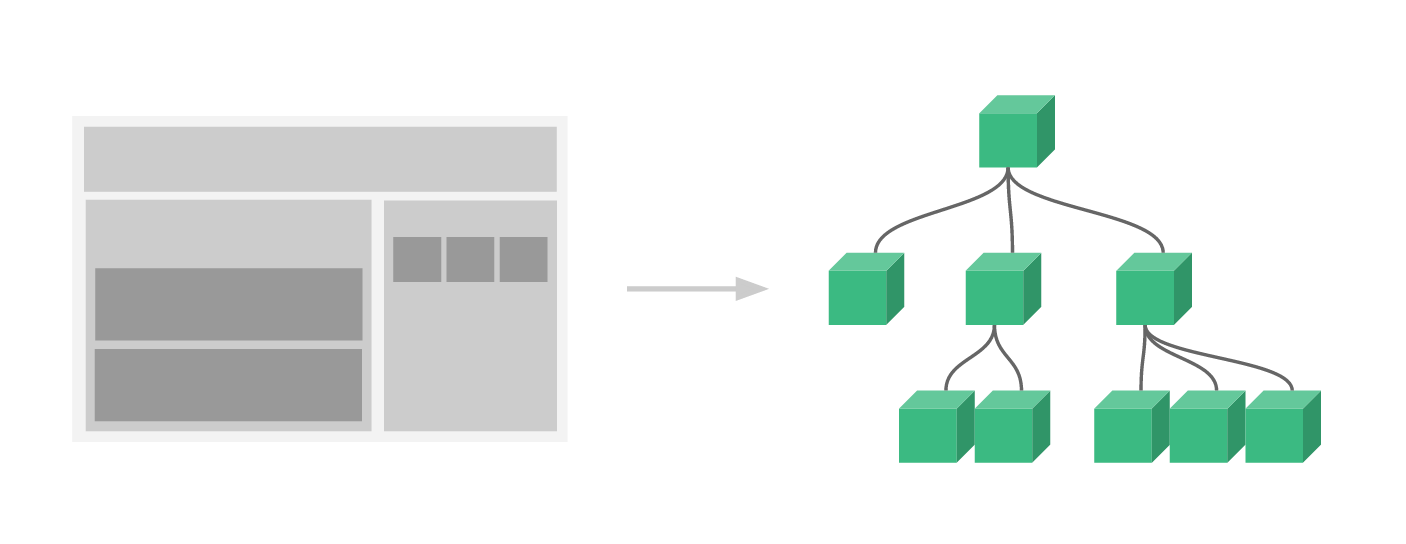
\includegraphics[scale=0.3]{pics/NestedComponentsTree.png}
    \caption{Darstellung von vernetzten Komponenten innerhalb einer Webpage}
        \small \url{https://vuejs.org/images/components.png?_sw-precache=b5c08269dfc26ae6d7db3801e9efd296}
    \label{fig:impl:NestedComponentsTree}
\end{figure}
Die folgende Grafik veranschaulicht den Component Tree, der zeigt wie die Single-Page Anwendung umgesetzt ist. 
Die grünen Boxen zeigen die miteinander vernetzten Komponenten, jeder Komponent kann mehrere Unterkomponenten haben, je nach Einteilung der Webseite.
\subsection{Angular vs. Vue}
\subsubsection{Marktstatistik}
\textbf{Angular:}
\begin{itemize}
    \item Angular wird eher für Seiten benutzt mit hohen Aufrufzahlen
    \item Nachdem was bekannt ist benutzen unter 0.4\% aller Webseiten Angular    
    \item Angular wird von 16.1\% Entwicklern weltweit verwendet \cite{AngVsVueSIM}
\end{itemize}

\textbf{Vue:}
\begin{itemize}
    \item Es gibt mehr als 1.523.449 Millionen Webseiten, die Vue benutzen
    \item Der Marktanteil von Vue beträgt nicht mehr als 0.5\% \cite{AngVsVueSIM}       
\end{itemize}
\subsubsection{Vor- und Nachteile}
Von der Lernkurve her ist Vue deutlich im Vorteil, da es einfacher zu verstehen ist als Angular. Angular benötigt viel Einarbeitungszeit, bis man die Funktionsweise
verstanden hat. Angular ist eher für umfangreiche Projekte gedacht, währenddessen Vue auf geringe Größe und hohe Performance abzielt. \\*
In Angular sind die Logik und das Aussehen strikt getrennt, währenddessen in Vue alles in einem File zu finden ist und mehr an HTML erinnert durch die Scripts, die man schreibt.
Ein Vorteil von Angular ist die Implementierung von Typescript, was eine Weiterentwicklung von JavaScript ist, die versucht die Macken von JavaScript zu verbessern.\\* 
Was noch zu erwägen ist ist, dass Angular weiter verbreitet ist als Vue und es oft Features oder Plugins gibt, die in Angular selbstverständlich sind, aber in Vue nicht aufzufinden sind.
Dies sollte sich aber im Laufe der Zeit verbessern. \\*  Generell kann man sagen, dass das Programmieren mit Angular eher and die Programmierung mit Java erinnert mit den Objekten, Abhängigkeiten,
Konstruktoren, usw. Während Vue an das Programmieren von Websites mittels HTML und JavaScript erinnert. \cite{AngVsVueHOST}
\subsubsection{Warum Vue?}
Unsere Entscheidung Vue zu nehmen ist einerseits von der Firma beeinflusst worden, da sie es vorgeschlagen haben und es bei ihnen das gängige Framework ist.\\*
Andere Faktoren waren noch, dass wir Angular in der Schule oft verwendet haben und wollten durch Vue eine andere Methode ausprobieren, um Webanwendungen zu erstellen.
Vue ist die bessere Wahl für den Umfang unserer Webanwendung gewesen und die bessere Performance in Vue ist wichtig, damit die Bestellungen reibungslos ablaufen können im Echtbetrieb.

\section{HTML}
\author{Benjamin Besic}
HTML genannt HyperText Markup Language, ist eine einheitliche, textbasierte, Auszeichnungssprache für Webdokumente. HTML definiert ganz allgemein gesehen die Struktur eines Dokuments. 
Am 13.März 1989 wurde am CERN in Genf das Konzept HTML von Tim Berners-Lee vorgeschlagen, um eine einheitliche Methode zu finden Dokumente öffentlich zu übermitteln. Seitdem ist HTML  einer Grundbausteine des World Wide Webs geworden. \\*
HTML basiert auf sogenannten Tags, die verschiedene Inhalte auf der Website definieren sollten. Diese basieren auf einer bestimmten Syntax, um das Schreiben zu vereinheitlichen. \\*
Es ist im Grunde eigentlich keine Programmiersprache, sondern eine statische Sprache, die zur Definierung benutzt wird. 
Das HTML Gerüst wird von einem Browser eingelesen und dieser generiert dann auf der Basis des HTML Files eine Website. \cite{HTMLTut} \cite{HTMLSeoKueche}

\begin{lstlisting}[language=HTML,caption=HTML File Grundgerüst,label=lst:impl:foo]
<!DOCTYPE html>
<html>
    <head>
        <title> Titel der Webseite </title>
    </head>
    <body>
        <h1> Ueberschrift </h1>
    </body>
</html>
\end{lstlisting}

Wie man im Beispiel sieht gibt bei Tags ein Beginn und ein Ende und der Inhalt dazwischen wird dargestellt.
Es gibt auch Tags ohne Beginn und Ende, sogenannte inhaltslose Tags.
Doch HTML wird meist nie allein verwendet, erst in der Kombination mit CSS, Bootstrap und JavaScript kann man eine gute Website erstellen.

\section{CSS}
\author{Benjamin Besic}
CSS (Cascading Style Sheets) ist die Sprache, die benutzt wird eine HTML Seite visuell zu gestalten. CSS ist wie HTML keine Programmiersprache, sie wurde dafür entwickelt um das Aussehen von HTML Seiten einheitlich zu verändern.\\*
Eine CSS-Datei wird durch einen Tag mit dem zugehörigen HTML Dokument verbunden und dadurch werden die Änderungen angewendet. \cite{CSSMozilla}

\begin{figure}[htp]
    \centering
    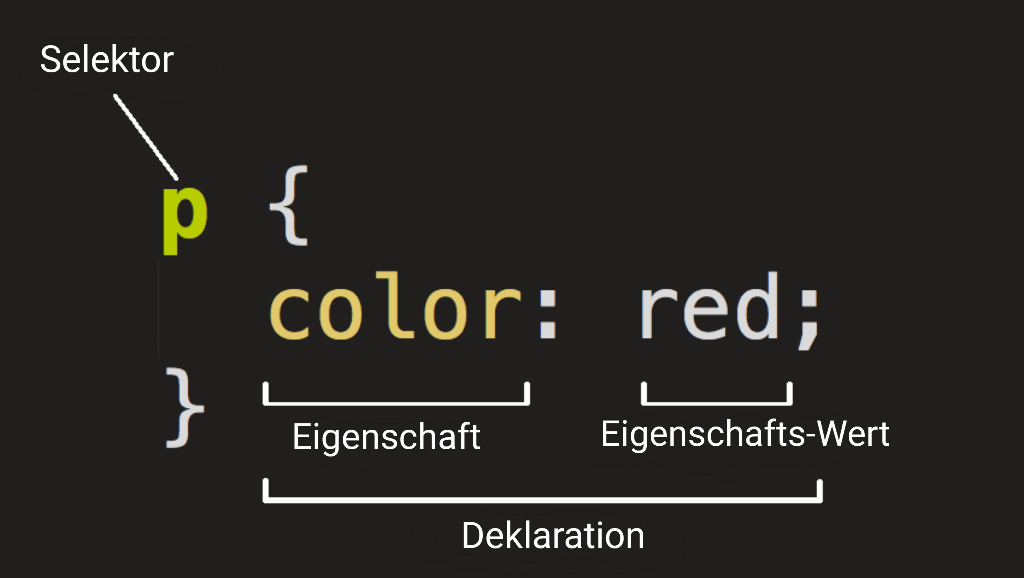
\includegraphics[scale=0.3]{pics/CSSRegel.png}
    \caption{Aufbau einer CSS-Regel}
        \small \url{https://media.prod.mdn.mozit.cloud/attachments/2017/09/27/15467/3889d04d90c10b27e863c6850d588c43/css-example.png}
    \label{fig:impl:CSSRule}
\end{figure}

Die Struktur von CSS-Dateien wird durch Regeln beschrieben. Jede Regel hat einen Selektor, der auf ein zugehöriges HTML Tag zugreift.
Innerhalb der Deklaration wird dann der Wert einer bestimmten Eigenschaft gesetzt (Mehrere Eigenschaften sind möglich).
Es gibt eine große Auswahl von Eigenschaften wie z.B.: Schriftfarbe, Textart, Positionierung, etc. \cite{CSSMozilla}

\section{JavaScript}
\author{Benjamin Besic}
JavaScript ist eine leichtgewichtige Skriptsprache, die 1995 vom Softwareunternehmen Netscape entwickelt geworden ist, um die Möglichkeiten von HTML und CSS zu erweitern.
Bekannt ist sie hauptsächlich als Sprache für Webseiten geworden, jedoch wird sie auch in vielen Umgebungen außerhalb des Browsers oft benutzt, wie z.B. Servern. 
\\* Sie unterstützt objektorientierte, imperative als auch deklarative Programmierung. JavaScript folgt dem Standard ECMAScript, welche alle Browser unterstützen. 
JavaScript dient dazu auf Webseiten Benutzerinteraktionen auszuwerten, Inhalte zu verändern, nachzuladen oder zu generieren. Sie bietet normalen HTML Webseiten eine Großzahl an Verbesserung, durch Hinzufügen von Programmierelementen. \\*
Jedoch sollte man JavaScript nicht mit der Programmiersprache Java verwechseln. Beide sind verschiedene Handelsmarken der Firma Oracle und ähneln einander höchstens mit der Syntax.
\cite{JSWiki} \cite{JSMozilla}
\section{JSON Web Token (JWT)}
\author{Benjamin Besic}
JSON Web Token ist ein nach RFC 7519 genormter Standard, um Daten sicher zwischen zwei Parteien auszutauschen. Es wird in der Form eines JSON-Objektes übertragen.
Die Information, die der Token enthält kann verifiziert werden, weil es eine digitale Unterschrift enthält. Der Token selbst kann entweder mit einem geheimen Schlüssel (HMAC-Algorithmus) oder einem private/public Schlüsselpaar (RSA oder ECDSA) verschlüsselt werden.\\*
Beliebte Anwendungsfälle des Tokens sind Authentifizierung und Datenaustausch. Der Token selbst enthält Informationen über den Absender und ob er die nötigen Zugriffsrechte hat.
\cite{JWTIO} \cite{JWTIONOS}
\subsection{Aufbau eines JWT}
Ein signierter JWT besteht aus 3 Teilen, getrennt durch einen Punkt. Jeder dieser Teile wird mit Base64 kodiert. \\*
Jeder JWT hat auch eine Gültigkeitsdauer, wenn diese abgelaufen ist, gilt ein Token als ungültig.
\clearpage
\begin{figure}[htp]
    \centering
    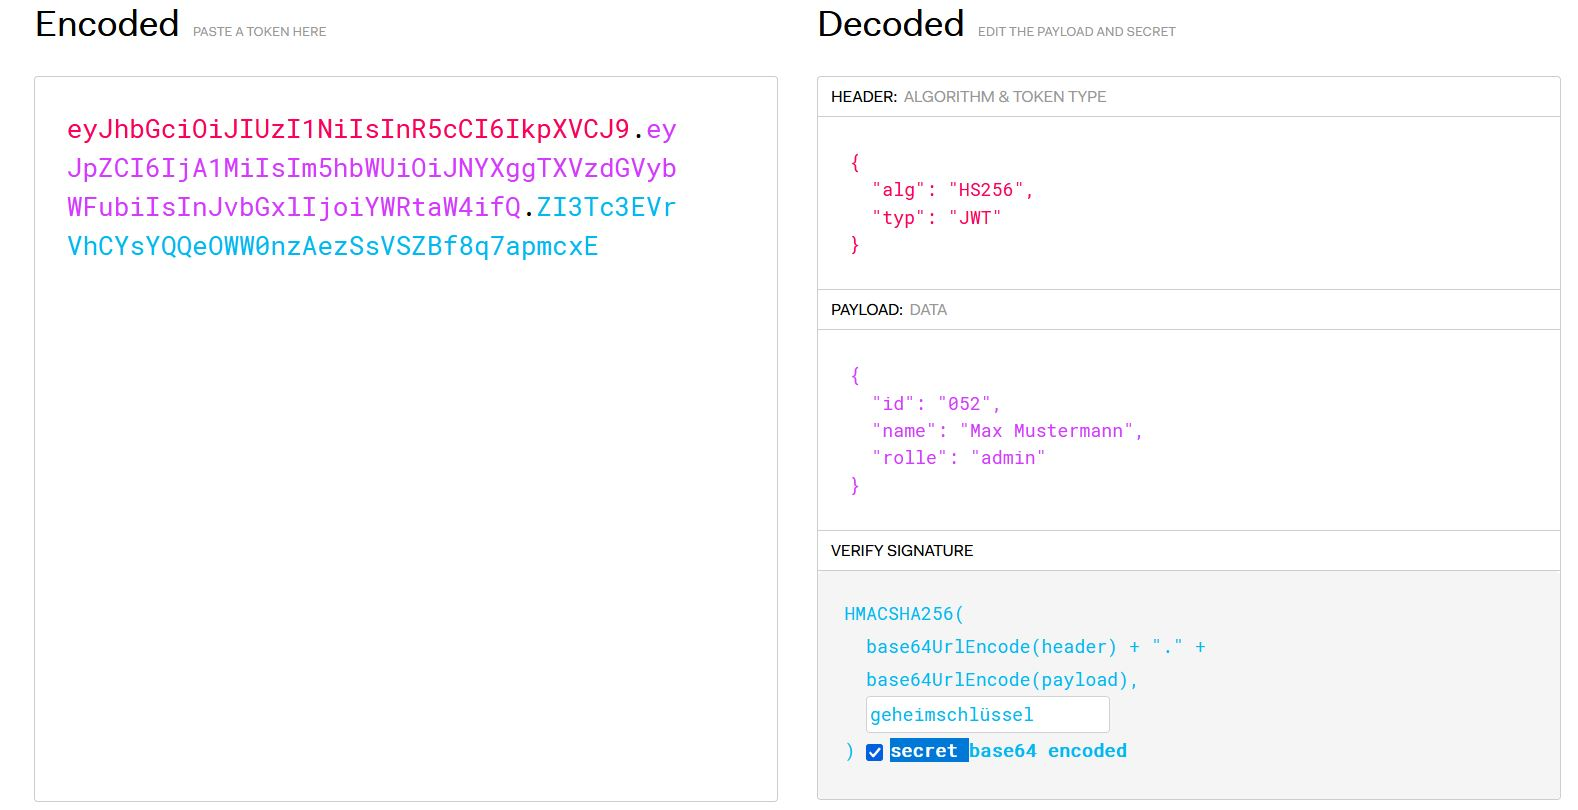
\includegraphics[scale=0.4]{pics/JWT.JPG}
    \caption{Aufbau eines JSON Web Tokens (Ausschnitt von jwt.io)}
        \small \url{https://jwt.io/}
    \label{fig:impl:JWT}
\end{figure}

\subsubsection{Header}
Der Header besteht meist aus zwei Teilen und liefert Informationen über den Typ des Tokens und den verwendeten Signatur- bzw. Verschlüsselungsalgorithmus.
\begin{itemize}
    \item Der "typ"-Wert beschreibt den IANA Medientypen des Tokens, oft wird "application/jwt" verwendet.
    \item Der "alg"-Wert gibt an welcher Algorithmus zum Signieren des Tokens verwendet wurde. Es ist möglich auch keine Verschlüsselung anzugeben, was jedoch nicht zu empfehlen ist. \cite{JWTIONOS}     
\end{itemize}
\subsubsection{Payload}
Der Payload ist der Teil des Tokens, der die tatsächlichen Daten bzw. Informationen enthält, die übermittelt werden sollen.
Sie werden als Key-/Value-Paare bereitgestellt, diese Werte werden bei JWT als Claims bezeichnet. \cite{JWTIONOS}  Davon gibt es drei verschiedene Arten:
\begin{itemize}
    \item \textbf{Registrierte Claims} sind standardisiert und im JWT Claim Register festgelegt. Es wird empfohlen diese zu verwenden.
    \item \textbf{Öffentliche Claims} sind nach belieben definierbar.
    \item \textbf{Private Claims} sind für Informationen gedacht, die speziell auf unsere Anwendung angepasst sind wie z.B. "Benutzer-ID". \cite{JWTIONOS} 
\end{itemize}

\subsubsection{Signature}
Diese wird durch Base64-Kodierung des Headers, des Payloads und der angegebenen Signaturmethode erzeugt. Der Aufbau ist definiert nach dem RFC 7515 Standard, auch genannt JWS (JSON Web Signature).
Damit die Signatur funktioniert, muss man einen geheimen Schlüssel verwenden, der nur dem Ursprung bekannt ist. \cite{JWTIONOS} 

\subsection{Sicherungsverfahren}
\subsubsection{Keine Sicherung}
Wenn die Daten keiner Verschlüsselung bedürfen, kann im Header "none" angegeben werden. In diesem Fall wird keine Signatur generiert, dadurch fällt auch der Signature-Teil weg. \\*
Ohne Sicherung lässt sich die Nachricht nach einer Base64-Entschlüsselung klar und deutlich lesen. Der Absender oder ob die Nachricht im Laufe verändert worden ist, ist nicht mehr verifizierbar.\cite{JWTIONOS} 
\subsubsection{Signatur (JWS)}
Im Normalfall reicht es nur zu prüfen, ob die Daten vom richtigen Absender kommen und ob Veränderungen geschehen sind. Da kommt die JWS (JSON Web Signature) zum Einsatz, die genau die vorher genannten Sachen überprüft.
\\* Bei diesem Verfahren lässt sich die Payload nach Base64-Entschlüsselung klar und deutlich lesen. \cite{JWTIONOS}
\subsubsection{Signatur (JWS) und Verschlüsselung (JWE)}
Es ist möglich zusätzlich zum JWS noch eine JWE (JSON Web Encryption) zu benützen. JWE verschlüsselt den Inhalt des Payloads, diese werden danach mit JWS signiert.
Um die Inhalte dann zu entschlüsseln wird noch ein Kennwort oder ein privater Schlüssel angegeben. \\*
Damit ist der Absender verifiziert, die Nachricht authentisch und der Payload ist nicht lesbar nach einer Base64-Entschlüsselung. \cite{JWTIONOS}
\section{Progressive Web App(PWA)}

\section{Google Charts}

\section{Jetpack Compose}

\section{Docker}
\subsection{Docker Compose}